% Options for packages loaded elsewhere
\PassOptionsToPackage{unicode}{hyperref}
\PassOptionsToPackage{hyphens}{url}
\documentclass[
]{article}
\usepackage{xcolor}
\usepackage[margin=1in]{geometry}
\usepackage{amsmath,amssymb}
\setcounter{secnumdepth}{5}
\usepackage{iftex}
\ifPDFTeX
  \usepackage[T1]{fontenc}
  \usepackage[utf8]{inputenc}
  \usepackage{textcomp} % provide euro and other symbols
\else % if luatex or xetex
  \usepackage{unicode-math} % this also loads fontspec
  \defaultfontfeatures{Scale=MatchLowercase}
  \defaultfontfeatures[\rmfamily]{Ligatures=TeX,Scale=1}
\fi
\usepackage{lmodern}
\ifPDFTeX\else
  % xetex/luatex font selection
\fi
% Use upquote if available, for straight quotes in verbatim environments
\IfFileExists{upquote.sty}{\usepackage{upquote}}{}
\IfFileExists{microtype.sty}{% use microtype if available
  \usepackage[]{microtype}
  \UseMicrotypeSet[protrusion]{basicmath} % disable protrusion for tt fonts
}{}
\makeatletter
\@ifundefined{KOMAClassName}{% if non-KOMA class
  \IfFileExists{parskip.sty}{%
    \usepackage{parskip}
  }{% else
    \setlength{\parindent}{0pt}
    \setlength{\parskip}{6pt plus 2pt minus 1pt}}
}{% if KOMA class
  \KOMAoptions{parskip=half}}
\makeatother
\usepackage{color}
\usepackage{fancyvrb}
\newcommand{\VerbBar}{|}
\newcommand{\VERB}{\Verb[commandchars=\\\{\}]}
\DefineVerbatimEnvironment{Highlighting}{Verbatim}{commandchars=\\\{\}}
% Add ',fontsize=\small' for more characters per line
\usepackage{framed}
\definecolor{shadecolor}{RGB}{248,248,248}
\newenvironment{Shaded}{\begin{snugshade}}{\end{snugshade}}
\newcommand{\AlertTok}[1]{\textcolor[rgb]{0.94,0.16,0.16}{#1}}
\newcommand{\AnnotationTok}[1]{\textcolor[rgb]{0.56,0.35,0.01}{\textbf{\textit{#1}}}}
\newcommand{\AttributeTok}[1]{\textcolor[rgb]{0.13,0.29,0.53}{#1}}
\newcommand{\BaseNTok}[1]{\textcolor[rgb]{0.00,0.00,0.81}{#1}}
\newcommand{\BuiltInTok}[1]{#1}
\newcommand{\CharTok}[1]{\textcolor[rgb]{0.31,0.60,0.02}{#1}}
\newcommand{\CommentTok}[1]{\textcolor[rgb]{0.56,0.35,0.01}{\textit{#1}}}
\newcommand{\CommentVarTok}[1]{\textcolor[rgb]{0.56,0.35,0.01}{\textbf{\textit{#1}}}}
\newcommand{\ConstantTok}[1]{\textcolor[rgb]{0.56,0.35,0.01}{#1}}
\newcommand{\ControlFlowTok}[1]{\textcolor[rgb]{0.13,0.29,0.53}{\textbf{#1}}}
\newcommand{\DataTypeTok}[1]{\textcolor[rgb]{0.13,0.29,0.53}{#1}}
\newcommand{\DecValTok}[1]{\textcolor[rgb]{0.00,0.00,0.81}{#1}}
\newcommand{\DocumentationTok}[1]{\textcolor[rgb]{0.56,0.35,0.01}{\textbf{\textit{#1}}}}
\newcommand{\ErrorTok}[1]{\textcolor[rgb]{0.64,0.00,0.00}{\textbf{#1}}}
\newcommand{\ExtensionTok}[1]{#1}
\newcommand{\FloatTok}[1]{\textcolor[rgb]{0.00,0.00,0.81}{#1}}
\newcommand{\FunctionTok}[1]{\textcolor[rgb]{0.13,0.29,0.53}{\textbf{#1}}}
\newcommand{\ImportTok}[1]{#1}
\newcommand{\InformationTok}[1]{\textcolor[rgb]{0.56,0.35,0.01}{\textbf{\textit{#1}}}}
\newcommand{\KeywordTok}[1]{\textcolor[rgb]{0.13,0.29,0.53}{\textbf{#1}}}
\newcommand{\NormalTok}[1]{#1}
\newcommand{\OperatorTok}[1]{\textcolor[rgb]{0.81,0.36,0.00}{\textbf{#1}}}
\newcommand{\OtherTok}[1]{\textcolor[rgb]{0.56,0.35,0.01}{#1}}
\newcommand{\PreprocessorTok}[1]{\textcolor[rgb]{0.56,0.35,0.01}{\textit{#1}}}
\newcommand{\RegionMarkerTok}[1]{#1}
\newcommand{\SpecialCharTok}[1]{\textcolor[rgb]{0.81,0.36,0.00}{\textbf{#1}}}
\newcommand{\SpecialStringTok}[1]{\textcolor[rgb]{0.31,0.60,0.02}{#1}}
\newcommand{\StringTok}[1]{\textcolor[rgb]{0.31,0.60,0.02}{#1}}
\newcommand{\VariableTok}[1]{\textcolor[rgb]{0.00,0.00,0.00}{#1}}
\newcommand{\VerbatimStringTok}[1]{\textcolor[rgb]{0.31,0.60,0.02}{#1}}
\newcommand{\WarningTok}[1]{\textcolor[rgb]{0.56,0.35,0.01}{\textbf{\textit{#1}}}}
\usepackage{graphicx}
\makeatletter
\newsavebox\pandoc@box
\newcommand*\pandocbounded[1]{% scales image to fit in text height/width
  \sbox\pandoc@box{#1}%
  \Gscale@div\@tempa{\textheight}{\dimexpr\ht\pandoc@box+\dp\pandoc@box\relax}%
  \Gscale@div\@tempb{\linewidth}{\wd\pandoc@box}%
  \ifdim\@tempb\p@<\@tempa\p@\let\@tempa\@tempb\fi% select the smaller of both
  \ifdim\@tempa\p@<\p@\scalebox{\@tempa}{\usebox\pandoc@box}%
  \else\usebox{\pandoc@box}%
  \fi%
}
% Set default figure placement to htbp
\def\fps@figure{htbp}
\makeatother
\setlength{\emergencystretch}{3em} % prevent overfull lines
\providecommand{\tightlist}{%
  \setlength{\itemsep}{0pt}\setlength{\parskip}{0pt}}
\usepackage[]{natbib}
\bibliographystyle{plainnat}
\usepackage{bookmark}
\IfFileExists{xurl.sty}{\usepackage{xurl}}{} % add URL line breaks if available
\urlstyle{same}
\hypersetup{
  pdftitle={Lab 03 - Nobel laureates},
  pdfauthor={Tina Huynh},
  hidelinks,
  pdfcreator={LaTeX via pandoc}}

\title{Lab 03 - Nobel laureates}
\author{Tina Huynh}
\date{}

\begin{document}
\maketitle

{
\setcounter{tocdepth}{2}
\tableofcontents
}
In January 2017, Buzzfeed published an article on why Nobel laureates
show immigration is so important for American science. You can read the
article
\href{https://www.buzzfeednews.com/article/peteraldhous/immigration-and-science}{here}.
In the article they show that while most living Nobel laureates in the
sciences are based in the US, many of them were born in other countries.
This is one reason why scientific leaders say that immigration is vital
for progress. In this lab we will work with the data from this article
to recreate some of their visualizations as well as explore new
questions.

\section{Learning goals}\label{learning-goals}

\begin{itemize}
\tightlist
\item
  Replicating published results
\item
  Data wrangling and visualisation
\end{itemize}

\section{Lab prep}\label{lab-prep}

Read the Buzzfeed article titled
\href{https://www.buzzfeednews.com/article/peteraldhous/immigration-and-science}{\emph{These
Nobel Prize Winners Show Why Immigration Is So Important For American
Science}}\emph{.} We will replicate this analysis in the workshop so
it's crucial that you're familiar with it ahead of time.

\section{Getting started}\label{getting-started}

Go to the course GitHub organization and locate your lab repo, which
should be named \texttt{lab-03-nobel-laureates-YOUR\_GITHUB\_USERNAME}.
Grab the URL of the repo, and clone it in RStudio. First, open the R
Markdown document \texttt{lab-03.Rmd} and Knit it. Make sure it compiles
without errors. The output will be in the file markdown \texttt{.md}
file with the same name.

\subsection{Warm up}\label{warm-up}

Before we introduce the data, let's warm up with some simple exercises.

\begin{itemize}
\tightlist
\item
  Update the YAML, changing the author name to your name, and
  \textbf{knit} the document.
\item
  Commit your changes with a meaningful commit message.
\item
  Push your changes to GitHub.
\item
  Go to your repo on GitHub and confirm that your changes are visible in
  your Rmd \textbf{and} md files. If anything is missing, commit and
  push again.
\end{itemize}

\subsection{Packages}\label{packages}

We'll use the \textbf{tidyverse} package for much of the data wrangling.
This package is already installed for you. You can load them by running
the following in your Console:

\begin{Shaded}
\begin{Highlighting}[]
\FunctionTok{library}\NormalTok{(tidyverse)}
\end{Highlighting}
\end{Shaded}

\subsection{Data}\label{data}

The dataset for this assignment can be found as a CSV (comma separated
values) file in the \texttt{data} folder of your repository. You can
read it in using the following.

\begin{Shaded}
\begin{Highlighting}[]
\NormalTok{nobel }\OtherTok{\textless{}{-}} \FunctionTok{read\_csv}\NormalTok{(}\StringTok{"data/nobel.csv"}\NormalTok{)}
\end{Highlighting}
\end{Shaded}

The variable descriptions are as follows:

\begin{itemize}
\tightlist
\item
  \texttt{id}: ID number
\item
  \texttt{firstname}: First name of laureate
\item
  \texttt{surname}: Surname
\item
  \texttt{year}: Year prize won
\item
  \texttt{category}: Category of prize
\item
  \texttt{affiliation}: Affiliation of laureate
\item
  \texttt{city}: City of laureate in prize year
\item
  \texttt{country}: Country of laureate in prize year
\item
  \texttt{born\_date}: Birth date of laureate
\item
  \texttt{died\_date}: Death date of laureate
\item
  \texttt{gender}: Gender of laureate
\item
  \texttt{born\_city}: City where laureate was born
\item
  \texttt{born\_country}: Country where laureate was born
\item
  \texttt{born\_country\_code}: Code of country where laureate was born
\item
  \texttt{died\_city}: City where laureate died
\item
  \texttt{died\_country}: Country where laureate died
\item
  \texttt{died\_country\_code}: Code of country where laureate died
\item
  \texttt{overall\_motivation}: Overall motivation for recognition
\item
  \texttt{share}: Number of other winners award is shared with
\item
  \texttt{motivation}: Motivation for recognition
\end{itemize}

In a few cases the name of the city/country changed after laureate was
given (e.g.~in 1975 Bosnia and Herzegovina was called the Socialist
Federative Republic of Yugoslavia). In these cases the variables below
reflect a different name than their counterparts without the suffix
`\_original`.

\begin{itemize}
\tightlist
\item
  \texttt{born\_country\_original}: Original country where laureate was
  born
\item
  \texttt{born\_city\_original}: Original city where laureate was born
\item
  \texttt{died\_country\_original}: Original country where laureate died
\item
  \texttt{died\_city\_original}: Original city where laureate died
\item
  \texttt{city\_original}: Original city where laureate lived at the
  time of winning the award
\item
  \texttt{country\_original}: Original country where laureate lived at
  the time of winning the award
\end{itemize}

\section{Exercises}\label{exercises}

\subsection{Get to know your data}\label{get-to-know-your-data}

\begin{enumerate}
\def\labelenumi{\arabic{enumi}.}
\tightlist
\item
  How many observations and how many variables are in the dataset? Use
  inline code to answer this question. What does each row represent?
\end{enumerate}

There are 935 observations and 26 variables in the dataset. Each row
represents a Nobel laureate.

There are some observations in this dataset that we will exclude from
our analysis to match the Buzzfeed results.

\begin{enumerate}
\def\labelenumi{\arabic{enumi}.}
\setcounter{enumi}{1}
\tightlist
\item
  Create a new data frame called \texttt{nobel\_living} that filters for
\end{enumerate}

\begin{itemize}
\tightlist
\item
  laureates for whom \texttt{country} is available
\item
  laureates who are people as opposed to organizations (organizations
  are denoted with \texttt{"org"} as their \texttt{gender})
\item
  laureates who are still alive (their \texttt{died\_date} is
  \texttt{NA})
\end{itemize}

\begin{Shaded}
\begin{Highlighting}[]
\NormalTok{nobel\_living }\OtherTok{\textless{}{-}}\NormalTok{ nobel }\SpecialCharTok{\%\textgreater{}\%}
  \FunctionTok{filter}\NormalTok{(}
    \SpecialCharTok{!}\FunctionTok{is.na}\NormalTok{(country),}
\NormalTok{    gender }\SpecialCharTok{!=} \StringTok{"org"}\NormalTok{,}
    \FunctionTok{is.na}\NormalTok{(died\_date)}
\NormalTok{  )}
\end{Highlighting}
\end{Shaded}

Confirm that once you have filtered for these characteristics you are
left with a data frame with 228 observations, once again using inline
code.

🧶 ✅ ⬆️ Knit, \emph{commit, and push your changes to GitHub with an
appropriate commit message. Make sure to commit and push all changed
files so that your Git pane is cleared up afterwards.}

\subsection{Most living Nobel laureates were based in the US when they
won their
prizes}\label{most-living-nobel-laureates-were-based-in-the-us-when-they-won-their-prizes}

\ldots{} says the Buzzfeed article. Let's see if that's true.

First, we'll create a new variable to identify whether the laureate was
in the US when they won their prize. We'll use the \texttt{mutate()}
function for this. The following pipeline mutates the
\texttt{nobel\_living} data frame by adding a new variable called
\texttt{country\_us}. We use an if statement to create this variable.
The first argument in the \texttt{if\_else()} function we're using to
write this if statement is the condition we're testing for. If
\texttt{country} is equal to \texttt{"USA"}, we set \texttt{country\_us}
to \texttt{"USA"}. If not, we set the \texttt{country\_us} to
\texttt{"Other"}.

\begin{Shaded}
\begin{Highlighting}[]
\NormalTok{Note that we can achieve the same result using the \textasciigrave{}fct\_other()\textasciigrave{} function we\textquotesingle{}ve seen before (i.e. with \textasciigrave{}country\_us = fct\_other(country, "USA")\textasciigrave{}). We decided to use the \textasciigrave{}if\_else()\textasciigrave{} here to show you one example of an if statement in R.}
\end{Highlighting}
\end{Shaded}

\begin{Shaded}
\begin{Highlighting}[]
\NormalTok{nobel\_living }\OtherTok{\textless{}{-}}\NormalTok{ nobel\_living }\SpecialCharTok{\%\textgreater{}\%}
  \FunctionTok{mutate}\NormalTok{(}
    \AttributeTok{country\_us =} \FunctionTok{if\_else}\NormalTok{(country }\SpecialCharTok{==} \StringTok{"USA"}\NormalTok{, }\StringTok{"USA"}\NormalTok{, }\StringTok{"Other"}\NormalTok{)}
\NormalTok{  )}
\end{Highlighting}
\end{Shaded}

Next, we will limit our analysis to only the following categories:
Physics, Medicine, Chemistry, and Economics.

\begin{Shaded}
\begin{Highlighting}[]
\NormalTok{nobel\_living\_science }\OtherTok{\textless{}{-}}\NormalTok{ nobel\_living }\SpecialCharTok{\%\textgreater{}\%}
  \FunctionTok{filter}\NormalTok{(category }\SpecialCharTok{\%in\%} \FunctionTok{c}\NormalTok{(}\StringTok{"Physics"}\NormalTok{, }\StringTok{"Medicine"}\NormalTok{, }\StringTok{"Chemistry"}\NormalTok{, }\StringTok{"Economics"}\NormalTok{))}
\end{Highlighting}
\end{Shaded}

For the next exercise work with the \texttt{nobel\_living\_science} data
frame you created above. This means you'll need to define this data
frame in your R Markdown document, even though the next exercise doesn't
explicitly ask you to do so.

\begin{enumerate}
\def\labelenumi{\arabic{enumi}.}
\setcounter{enumi}{2}
\item
  Create a faceted bar plot visualizing the relationship between the
  category of prize and whether the laureate was in the US when they won
  the nobel prize. Interpret your visualization, and say a few words
  about whether the Buzzfeed headline is supported by the data.

  \begin{itemize}
  \tightlist
  \item
    Your visualization should be faceted by category.
  \item
    For each facet you should have two bars, one for winners in the US
    and one for Other.
  \item
    Flip the coordinates so the bars are horizontal, not vertical.
  \end{itemize}
\end{enumerate}

\begin{Shaded}
\begin{Highlighting}[]
\FunctionTok{ggplot}\NormalTok{(nobel\_living\_science, }\FunctionTok{aes}\NormalTok{(}\AttributeTok{x =}\NormalTok{ country\_us)) }\SpecialCharTok{+}
  \FunctionTok{geom\_bar}\NormalTok{() }\SpecialCharTok{+}
  \FunctionTok{facet\_wrap}\NormalTok{(}\SpecialCharTok{\textasciitilde{}}\NormalTok{ category) }\SpecialCharTok{+}
  \FunctionTok{coord\_flip}\NormalTok{() }\SpecialCharTok{+}
  \FunctionTok{labs}\NormalTok{(}
    \AttributeTok{x =} \StringTok{"Country"}\NormalTok{,}
    \AttributeTok{y =} \StringTok{"Number of Nobel Laureates"}\NormalTok{,}
    \AttributeTok{title =} \StringTok{"Nobel Laureates by Category and Country"}
\NormalTok{  )}
\end{Highlighting}
\end{Shaded}

\pandocbounded{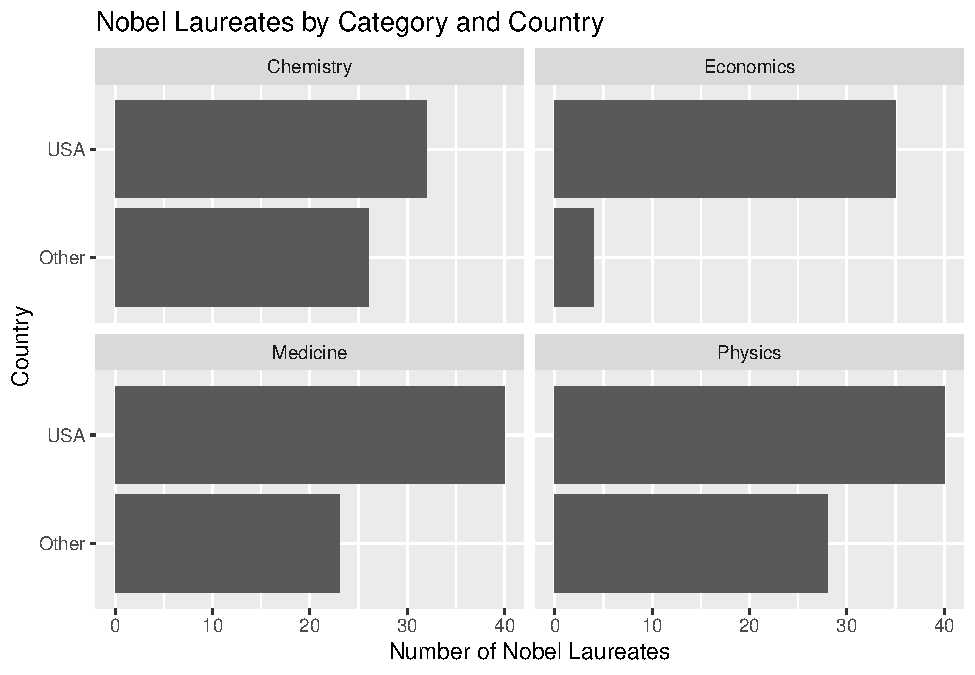
\includegraphics[keepaspectratio]{lab-03-nobel-laureates_files/figure-latex/faceted-bar-plot-1.pdf}}

The visualization shows that the majority of living Nobel laureates in
Physics, Chemistry, Medicine, and Economics were indeed based in the US
when they won their prizes. This supports the Buzzfeed headline's claim.

🧶 ✅ ⬆️ Knit, \emph{commit, and push your changes to GitHub with an
appropriate commit message. Make sure to commit and push all changed
files so that your Git pane is cleared up afterwards.d}

\subsection{But of those US-based Nobel laureates, many were born in
other
countries}\label{but-of-those-us-based-nobel-laureates-many-were-born-in-other-countries}

\begin{Shaded}
\begin{Highlighting}[]
\NormalTok{**Hint:** You should be able to borrow from code you used earlier to create the \textasciigrave{}country\_us\textasciigrave{} variable.}
\end{Highlighting}
\end{Shaded}

\begin{enumerate}
\def\labelenumi{\arabic{enumi}.}
\setcounter{enumi}{3}
\tightlist
\item
  Create a new variable called \texttt{born\_country\_us} that has the
  value \texttt{"USA"} if the laureate is born in the US, and
  \texttt{"Other"} otherwise. How many of the winners are born in the
  US?
\end{enumerate}

\begin{Shaded}
\begin{Highlighting}[]
\NormalTok{nobel\_living\_science }\OtherTok{\textless{}{-}}\NormalTok{ nobel\_living\_science }\SpecialCharTok{\%\textgreater{}\%}
  \FunctionTok{mutate}\NormalTok{(}
    \AttributeTok{born\_country\_us =} \FunctionTok{if\_else}\NormalTok{(born\_country }\SpecialCharTok{==} \StringTok{"USA"}\NormalTok{, }\StringTok{"USA"}\NormalTok{, }\StringTok{"Other"}\NormalTok{)}
\NormalTok{  )}

\CommentTok{\# Count winners born in the US}
\NormalTok{us\_born\_count }\OtherTok{\textless{}{-}}\NormalTok{ nobel\_living\_science }\SpecialCharTok{\%\textgreater{}\%}
  \FunctionTok{filter}\NormalTok{(born\_country\_us }\SpecialCharTok{==} \StringTok{"USA"}\NormalTok{) }\SpecialCharTok{\%\textgreater{}\%}
  \FunctionTok{nrow}\NormalTok{()}
\end{Highlighting}
\end{Shaded}

There are 105 winners who were born in the US.

\begin{enumerate}
\def\labelenumi{\arabic{enumi}.}
\setcounter{enumi}{4}
\item
  Add a second variable to your visualization from Exercise 3 based on
  whether the laureate was born in the US or not. Based on your
  visualization, do the data appear to support Buzzfeed's claim? Explain
  your reasoning in 1-2 sentences.

  \begin{itemize}
  \tightlist
  \item
    Your final visualization should contain a facet for each category.
  \item
    Within each facet, there should be a bar for whether the laureate
    won the award in the US or not.
  \item
    Each bar should have segments for whether the laureate was born in
    the US or not.
  \end{itemize}
\end{enumerate}

\begin{Shaded}
\begin{Highlighting}[]
\FunctionTok{ggplot}\NormalTok{(nobel\_living\_science, }\FunctionTok{aes}\NormalTok{(}\AttributeTok{x =}\NormalTok{ country\_us, }\AttributeTok{fill =}\NormalTok{ born\_country\_us)) }\SpecialCharTok{+}
  \FunctionTok{geom\_bar}\NormalTok{() }\SpecialCharTok{+}
  \FunctionTok{facet\_wrap}\NormalTok{(}\SpecialCharTok{\textasciitilde{}}\NormalTok{ category) }\SpecialCharTok{+}
  \FunctionTok{coord\_flip}\NormalTok{() }\SpecialCharTok{+}
  \FunctionTok{labs}\NormalTok{(}
    \AttributeTok{x =} \StringTok{"Country where award was won"}\NormalTok{,}
    \AttributeTok{y =} \StringTok{"Number of Nobel Laureates"}\NormalTok{,}
    \AttributeTok{fill =} \StringTok{"Birth country"}\NormalTok{,}
    \AttributeTok{title =} \StringTok{"Nobel Laureates by Category, Award Country, and Birth Country"}
\NormalTok{  ) }\SpecialCharTok{+}
  \FunctionTok{scale\_fill\_manual}\NormalTok{(}\AttributeTok{values =} \FunctionTok{c}\NormalTok{(}\StringTok{"USA"} \OtherTok{=} \StringTok{"\#4e79a7"}\NormalTok{, }\StringTok{"Other"} \OtherTok{=} \StringTok{"\#f28e2c"}\NormalTok{))}
\end{Highlighting}
\end{Shaded}

\pandocbounded{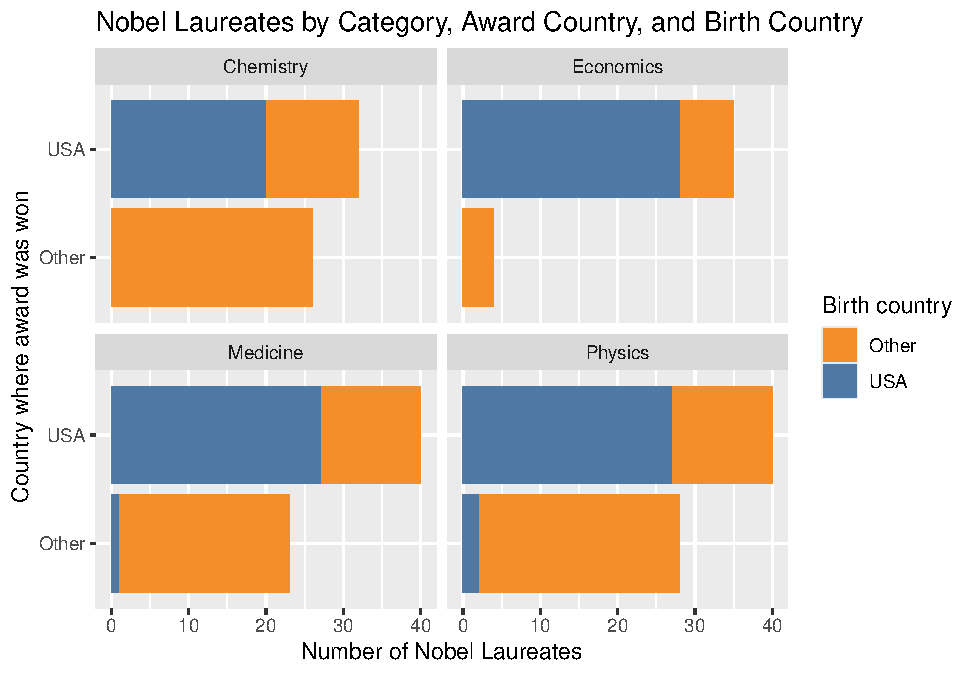
\includegraphics[keepaspectratio]{lab-03-nobel-laureates_files/figure-latex/stacked-bar-plot-1.pdf}}

The data supports Buzzfeed's claim. While many Nobel laureates were
based in the US when they won their prizes, a substantial portion of
these US-based winners were actually born in other countries,
highlighting the importance of immigration to American scientific
achievement.

🧶 ✅ ⬆️ Knit, \emph{commit, and push your changes to GitHub with an
appropriate commit message. Make sure to commit and push all changed
files so that your Git pane is cleared up afterwards.}

\subsection{Here's where those immigrant Nobelists were
born}\label{heres-where-those-immigrant-nobelists-were-born}

\begin{Shaded}
\begin{Highlighting}[]
\NormalTok{Note that your bar plot won\textquotesingle{}t exactly match the one from the Buzzfeed article. This is likely because the data has been updated since the article was published.}
\end{Highlighting}
\end{Shaded}

\begin{enumerate}
\def\labelenumi{\arabic{enumi}.}
\setcounter{enumi}{5}
\tightlist
\item
  In a single pipeline, filter for laureates who won their prize in the
  US, but were born outside of the US, and then create a frequency table
  (with the \texttt{count()} function) for their birth country
  (\texttt{born\_country}) and arrange the resulting data frame in
  descending order of number of observations for each country. Which
  country is the most common?
\end{enumerate}

\begin{Shaded}
\begin{Highlighting}[]
\NormalTok{immigrant\_nobelists }\OtherTok{\textless{}{-}}\NormalTok{ nobel\_living\_science }\SpecialCharTok{\%\textgreater{}\%}
  \FunctionTok{filter}\NormalTok{(country\_us }\SpecialCharTok{==} \StringTok{"USA"}\NormalTok{, born\_country\_us }\SpecialCharTok{==} \StringTok{"Other"}\NormalTok{) }\SpecialCharTok{\%\textgreater{}\%}
  \FunctionTok{count}\NormalTok{(born\_country) }\SpecialCharTok{\%\textgreater{}\%}
  \FunctionTok{arrange}\NormalTok{(}\FunctionTok{desc}\NormalTok{(n))}

\CommentTok{\# Display the table}
\NormalTok{immigrant\_nobelists}
\end{Highlighting}
\end{Shaded}

\begin{verbatim}
## # A tibble: 21 x 2
##    born_country       n
##    <chr>          <int>
##  1 Germany            7
##  2 United Kingdom     7
##  3 China              5
##  4 Canada             4
##  5 Japan              3
##  6 Australia          2
##  7 Israel             2
##  8 Norway             2
##  9 Austria            1
## 10 Finland            1
## # i 11 more rows
\end{verbatim}

The most common birth country for immigrant Nobel laureates who won
their prize while in the US is Germany.

🧶 ✅ ⬆️ Knit, \emph{commit, and push your changes to GitHub with an
appropriate commit message. Make sure to commit and push all changed
files so that your Git pane is cleared up afterwards and review the md
document on GitHub to make sure you're happy with the final state of
your work.}

Now go back through your write up to make sure you've answered all
questions and all of your R chunks are properly labeled. Once you decide
that you are done with the lab, choose the knit drop down and select
\texttt{Knit\ to\ tufte\_handout} to generate a pdf. Download and submit
that pdf to Canvas.

\section{Interested in how Buzzfeed made their
visualizations?}\label{interested-in-how-buzzfeed-made-their-visualizations}

The plots in the Buzzfeed article are called waffle plots. You can find
the code used for making these plots in Buzzfeed's GitHub repo (yes,
they have one!)
\href{https://buzzfeednews.github.io/2017-01-immigration-and-science/}{here}.
You're not expected to recreate them as part of your assignment, but
you're welcomed to do so for fun!

\end{document}
